\documentclass[a4paper]{article}
\usepackage{vntex}
%\usepackage[english,vietnam]{babel}
%\usepackage[utf8]{inputenc}

%\usepackage[utf8]{inputenc}
%\usepackage[francais]{babel}
\usepackage{a4wide,amssymb,epsfig,latexsym,multicol,array,hhline,fancyhdr,pictex, latexsym, graphicx,amsbsy,amsfonts,amsthm,verbatim}
\usepackage{amsmath}
\usepackage{lastpage}
\usepackage[lined,boxed,commentsnumbered]{algorithm2e}
\usepackage{enumerate}
\usepackage{color}
\usepackage{graphicx}							% Standard graphics package
\usepackage{array}
\usepackage{indentfirst}
\usepackage{tabularx, caption}
\usepackage{multirow}
\usepackage{multicol}
\usepackage{rotating}
\usepackage{graphics}
\usepackage{geometry}
\usepackage{setspace}
\usepackage{epsfig}
\usepackage{tikz}
\usepackage{pgfplots}
\usepackage{tikz-timing}[2014/10/29]
\usetikztiminglibrary[rising arrows]{clockarrows}
\usepackage{xparse} % NewDocumentCommand, IfValueTF, IFBooleanTF
\usetikzlibrary{arrows,snakes,backgrounds}
\usepackage{hyperref}
\usetikzlibrary{arrows,shapes.gates.logic.US,shapes.gates.logic.IEC,calc}
\hypersetup{urlcolor=blue,linkcolor=black,citecolor=black,colorlinks=true} 
\usepackage{footnote}
\usetikzlibrary{patterns}
\usepackage[]{algorithm2e}
\usepackage{xcolor}

\usepackage{listings}
\usepackage{color}
\definecolor{lightgray}{gray}{0.9}

\newcommand{\PreserveBackslash}[1]{\let\temp=\\#1\let\\=\temp}
\newcolumntype{C}[1]{>{\PreserveBackslash\centering}p{#1}}
\newcolumntype{R}[1]{>{\PreserveBackslash\raggedleft}p{#1}}
\newcolumntype{L}[1]{>{\PreserveBackslash\raggedright}p{#1}}


\newcommand{\inlinecode}[2]{\colorbox{lightgray}{\lstinline[language=#1] $#2$}}


% the following is needed for syntax highlighting

\definecolor{dkgreen}{rgb}{0,0.6,0}
\definecolor{gray}{rgb}{0.5,0.5,0.5}
\definecolor{mauve}{rgb}{01,0,0.82}

\lstset{ %
  language=[Sharp]C,       % the language of the code
  basicstyle=\tt\footnotesize,        % the size of the fonts that are used for the code
  numbers=left,                   % where to put the line-numbers
  numberstyle=\tiny\color{gray},  % the style that is used for the line-numbers
  stepnumber=2,                   % the step between two line-numbers. If it's 1, each line 
                                  % will be numbered
  numbersep=5pt,                  % how far the line-numbers are from the code
  backgroundcolor=\color{white},  % choose the background color. You must add \usepackage{color}
  showspaces=false,               % show spaces adding particular underscores
  showstringspaces=false,         % underline spaces within strings
  showtabs=false,                 % show tabs within strings adding particular underscores
  frame=single,                   % adds a frame around the code
  rulecolor=\color{black},        % if not set, the frame-color may be changed on line-breaks within not-black text (e.g. commens (green here))
  tabsize=2,                      % sets default tabsize to 2 spaces
  captionpos=b,                   % sets the caption-position to bottom
  breaklines=true,                % sets automatic line breaking
  breakatwhitespace=false,        % sets if automatic breaks should only happen at whitespace
  title=\lstname,                 % show the filename of files included with \lstinputlisting;
                                  % also try caption instead of title
  keywordstyle=\color{blue},          % keyword style
  commentstyle=\color{dkgreen},       % comment style
  stringstyle=\color{mauve},         % string literal style
  escapeinside={\%*}{*)},            % if you want to add a comment within your code
  morekeywords={*, ...},              % if you want to add more keywords to the set
}

\usepackage{xcolor,pifont}
\newcommand*\colourcheck[1]{%
  \expandafter\newcommand\csname #1check\endcsname{\textcolor{#1}{\ding{51}}}%
}
\colourcheck{blue}
\colourcheck{green}
\colourcheck{red}

\NewDocumentCommand{\busref}{som}{\texttt{%
#3%
\IfValueTF{#2}{[#2]}{}%
\IfBooleanTF{#1}{\#}{}%
}}


\usetikzlibrary{arrows,snakes,backgrounds}
\usepackage{hyperref}
\hypersetup{urlcolor=blue,linkcolor=black,citecolor=black,colorlinks=true} 

\newtheorem{theorem}{{\bf Định lý}}
\newtheorem{property}{{\bf Tính chất}}
\newtheorem{proposition}{{\bf Mệnh đề}}
\newtheorem{corollary}[proposition]{{\bf Hệ quả}}
\newtheorem{lemma}[proposition]{{\bf Bổ đề}}


%\usepackage{fancyhdr}
\setlength{\headheight}{40pt}
\pagestyle{fancy}
\fancyhead{} % clear all header fields
\fancyhead[L]{
 \begin{tabular}{rl}
    \begin{picture}(25,15)(0,0)
    \put(0,-8){
\includegraphics[width=8mm, height=8mm]{hcmut.png}}
    %\put(0,-8){\epsfig{width=10mm,figure=hcmut.eps}}
   \end{picture}&
	%
\includegraphics[width=8mm, height=8mm]{hcmut.png} & %
	\begin{tabular}{l}
		\textbf{\bf \ttfamily Trường Đại Học Bách Khoa Tp.Hồ Chí Minh}\\
		\textbf{\bf \ttfamily Khoa Khoa Học và Kỹ Thuật Máy Tính}
	\end{tabular} 	
 \end{tabular}
}
\fancyhead[R]{
	\begin{tabular}{l}
		\tiny \bf \\
		\tiny \bf 
	\end{tabular}  }
\fancyfoot{} % clear all footer fields
\fancyfoot[L]{\scriptsize \ttfamily Assignment 1 - Computer Network - Semester 191} %%%%% HERE
\fancyfoot[R]{\scriptsize \ttfamily Trang {\thepage}/\pageref{LastPage}}
\renewcommand{\headrulewidth}{0.3pt}
\renewcommand{\footrulewidth}{0.3pt}
\renewcommand{\baselinestretch}{1.5}


%%%
\setcounter{secnumdepth}{4}
\setcounter{tocdepth}{3}
\makeatletter
\newcounter {subsubsubsection}[subsubsection]
\renewcommand\thesubsubsubsection{\thesubsubsection .\@alph\c@subsubsubsection}
\newcommand\subsubsubsection{\@startsection{subsubsubsection}{4}{\z@}%
                                     {-3.25ex\@plus -1ex \@minus -.2ex}%
                                     {1.5ex \@plus .2ex}%
                                     {\normalfont\normalsize\bfseries}}
\newcommand*\l@subsubsubsection{\@dottedtocline{3}{10.0em}{4.1em}}
\newcommand*{\subsubsubsectionmark}[1]{}
\makeatother

\usepackage{tocloft}

\newcommand{\listhistogramname}{\large{Danh sách Biểu đồ}}
\newlistof{histogram}{exp}{\listhistogramname}
\newcommand{\histogram}[1]{%
\refstepcounter{histogram}
\par\noindent\textbf{Histogram \thehistogram. #1}
\addcontentsline{exp}{histogram}
{\protect\numberline{\thehistogram}#1}\par}

\graphicspath{{./images/}}

\begin{document}

\begin{titlepage}
\begin{center}
\Large{ĐẠI HỌC QUỐC GIA THÀNH PHỐ HỒ CHÍ MINH \\
TRƯỜNG ĐẠI HỌC BÁCH KHOA \\
KHOA KHOA HỌC - KỸ THUẬT MÁY TÍNH }
\end{center}


\begin{figure}[h!]
\begin{center}

\includegraphics[width=5cm]{hcmut.png}
\end{center}
\end{figure}

\begin{center}
\begin{tabular}{c}
\multicolumn{1}{l}{\textbf{{\Large Mạng Máy Tính - Computer Network - 191}}}\\		%%%%% HERE
~~\\
\hline
\\
\multicolumn{1}{l}{\textbf{{\Large  Assignment 1}}}\\
\\
\textsc{{\huge{Socket Chat Application}}}\\ % TODO: Change here for customing your lab.
\\
\hline
\end{tabular}
\end{center}

\begin{table}[h]
{\textsc {\large
\begin{tabular}{rrl}
\hspace{5 cm} & GVHD: & PhD. Phạm Trần Vũ\\
& & PhD. Nguyễn Mạnh Thìn \\
& Sinh Viên: &  \\
& & Hoàng Vũ Trọng Thụy - 1710321 \\
& & Lê Trung Vinh - \\
\end{tabular}
}}
\end{table}
\end{titlepage}

\newpage
\tableofcontents
\newpage
\listoffigures
\newpage

\section{Định nghĩa chức năng}
	\subsection{Đăng nhập}
	\begin{itemize}
		\item Cho phép user nhập tên và nhập đường dẫn tới server và tên port để vào phòng chat. Tên user phải bắt đầu bằng chữ cái
		\item Tạo avatar là chữ cái đầu tên của user
	\end{itemize}
	\subsection{Nhắn tin giữa 2 user với nhau}
	\begin{itemize}
		\item Cho phép 2 user trong phòng chat nhắn tin qua lại với nhau.
		\item Tin nhắn gửi đi có thể là tin nhắn văn bản hoặc tin nhắn thoại.
		\item User có thể đổi màu tin nhắn
	\end{itemize}
	\subsection{Giao tiếp giữa 1 user với các user khác trong phòng chat}
	\begin{itemize}
		\item Cho phép user gửi tin nhắn đến cùng lúc các user khác thông qua một kênh chat chung.
		\item Tin nhắn gửi đi có thể là tin nhắn văn bản hoặc tin nhắn thoại.
	\end{itemize}
	\subsection{Gửi file}
	\begin{itemize}
		\item Cho phép user gửi một tệp tin từ trong máy tính cá nhân tới các user khác trong phòng chat chung hoặc tới một user khác trong server.
	\end{itemize}
	\subsection{Xem trạng thái online offline của bạn bè trong list danh sách}
	\begin{itemize}
		\item User có thể thấy ai đang online nếu người đó có tích xanh trước tên của mình, offline nếu tích xám ở bảng danh sách user và away nếu tích có màu vàng.
		\item User cũng có thể đổi trạng thái sử dụng của mình về online, offline, away.
	\end{itemize}
	\subsection{Server}
	\begin{itemize}
		\item Là nơi xử lý các hoạt động của user như đăng nhập, gửi tin nhắn, gửi file, chuyển trạng thái, chuyển kênh
		\item Server có 2 phiên bản CLI và UI tùy sở thích người dùng.
	\end{itemize}

\section{Định nghĩa giao thức}

\section{Miêu tả chi tiết hiện thực}

\section{Thiết kế chi tiết}

\section{Kết quả và đánh giá}

\section{Hướng dẫn sử dụng}
	    \subsection{Bước 1: Khởi động server}
	Cách 1: sử dụng server CLI:
	\begin{itemize}
		\item Chạy class com.server.Server.
		\newline
		\begin{figure}[H]
			\centering
			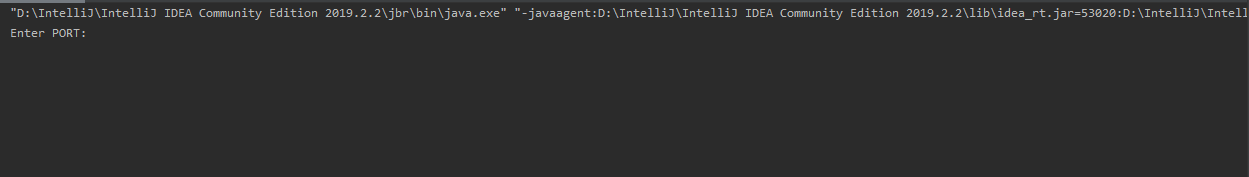
\includegraphics[width=\linewidth]{server_CLI.PNG}
			\caption{Server CLI}
			\label{fig:my_label}
		\end{figure}
		\item Nhập tên port vào. VD: 9001.
	\end{itemize}
	Cách 2: sử dụng server UI:
	\begin{itemize}
		\item Chạy class com.server.ServerController.
		\newline
		\begin{figure}[H]
			\centering
			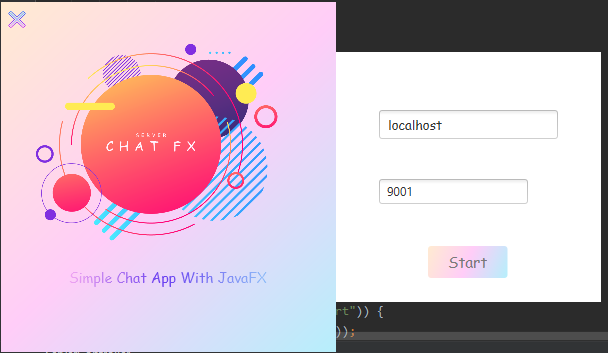
\includegraphics[scale=0.5]{server_Launcher.PNG}
			\caption{Server UI}
			\label{fig:my_label}
		\end{figure}
		\item Nhập đường dẫn vào server ở ô localhost. Nhập port vào ô dưới rồi bấm nút Start để khởi động server.
		\item Để tắt server nhấn nút stop
		\begin{figure}[H]
			\centering
			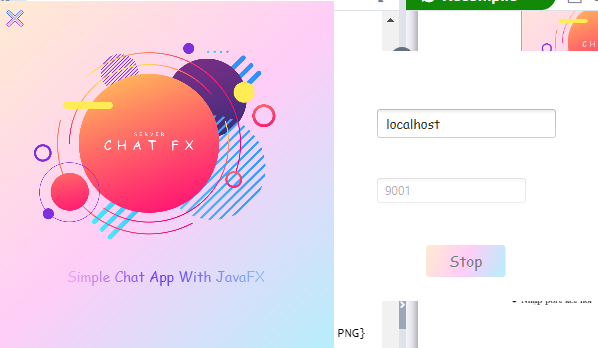
\includegraphics[scale = 0.5]{stop-server.PNG}
			\caption{Server CLI}
			\label{fig:my_label}
		\end{figure}
	\end{itemize}
	\subsection{Bước 2: Đăng nhập}
	Chạy class com.client.login.Mainlauncher.
	\newline
	\begin{figure}[H]
		\centering
		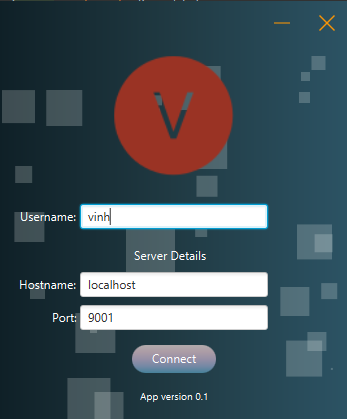
\includegraphics[scale=0.5]{LogIn.PNG}
		\caption{Màn hình Login}
		\label{fig:my_label}
	\end{figure}
	
	\begin{itemize}
		\item Nhập tên người dùng vào ô username.
		\item Nhập đường dẫn tới server vào hostname.
		\item Nhập port kết nối.
	\end{itemize}
	Giao diện sau khi đăng nhập thành công vào server.
	\begin{figure}[H]
		\centering
		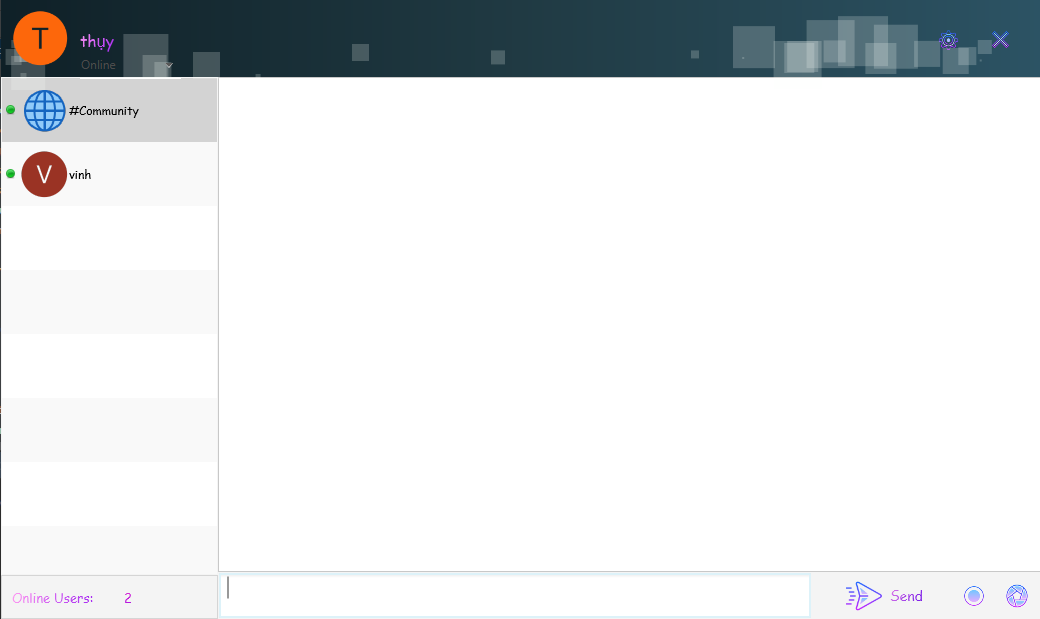
\includegraphics[scale=0.5]{interface.PNG}
		\caption{Main Interface}
		\label{fig:my_label}
	\end{figure}
	\subsection{Bước 3: Gửi tin nhắn}
	\subsubsection{Gửi tin nhắn vào phòng chat chung}
	\begin{itemize}
		\item Nhấn chọn kênh chat community
		\item Nhập tin nhắn từ bàn phím vào ô chat dưới cùng
		\begin{figure}[H]
			\centering
			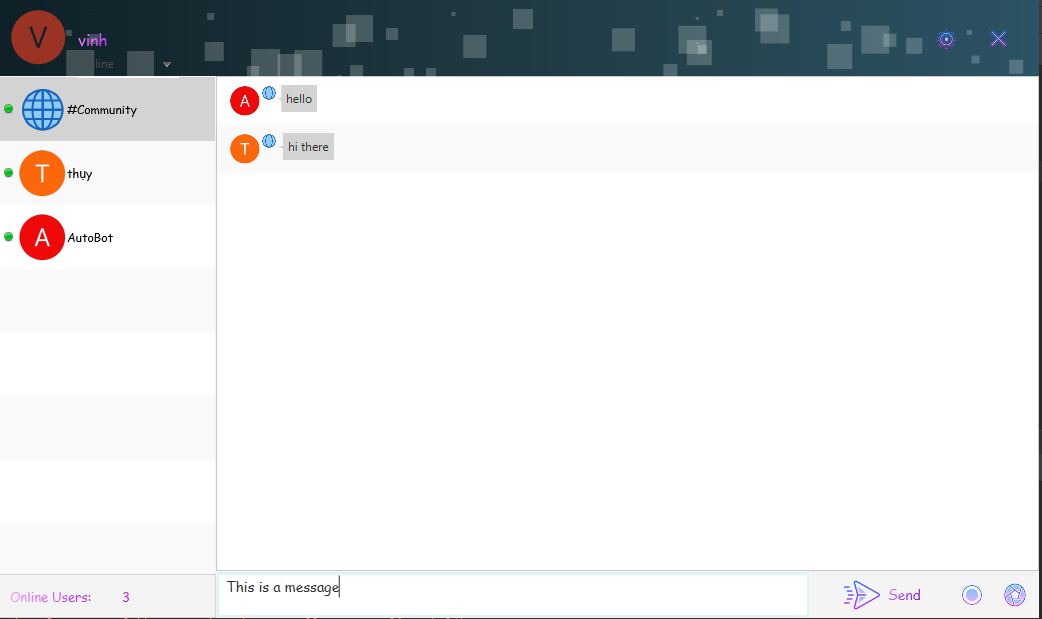
\includegraphics[scale=0.5]{enter-message.PNG}
			\caption{Send public message}
			\label{fig:my_label}
		\end{figure}
		\item Bấm enter hoặc nhấn nút send cạnh ô chat sẽ được kết quả như hình
		\begin{figure}[H]
			\centering
			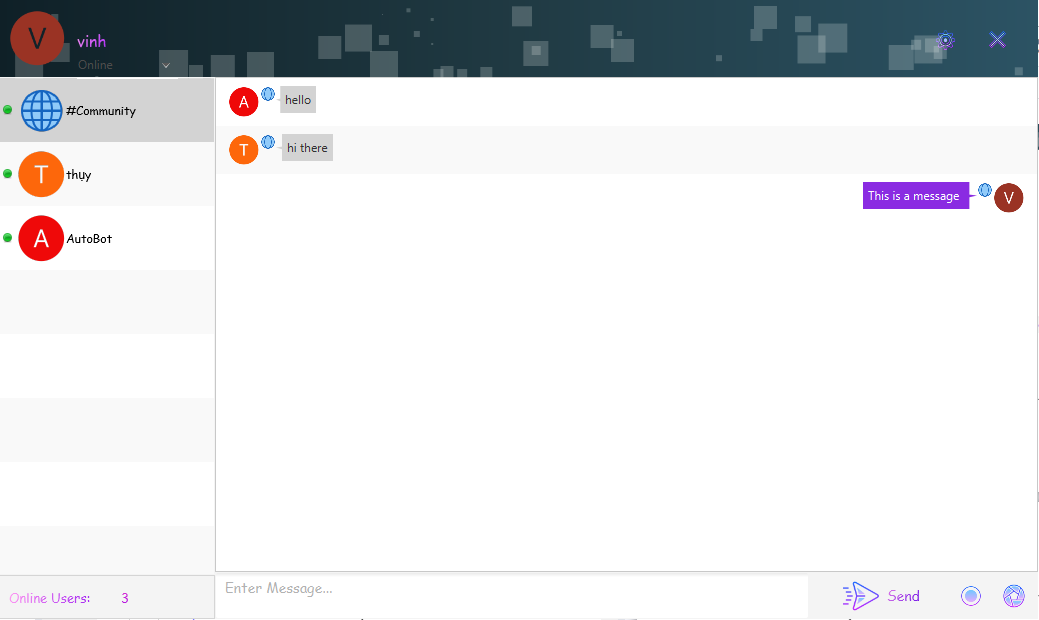
\includegraphics[scale=0.5]{message-sent.PNG}
			\caption{Message sent in community channel}
			\label{fig:my_label}
		\end{figure}
		\item Để gửi tin nhắn thoại nhấn vào nút thu âm bên phải nút send và bắt đầu nói.
		\begin{figure}[H]
			\centering
			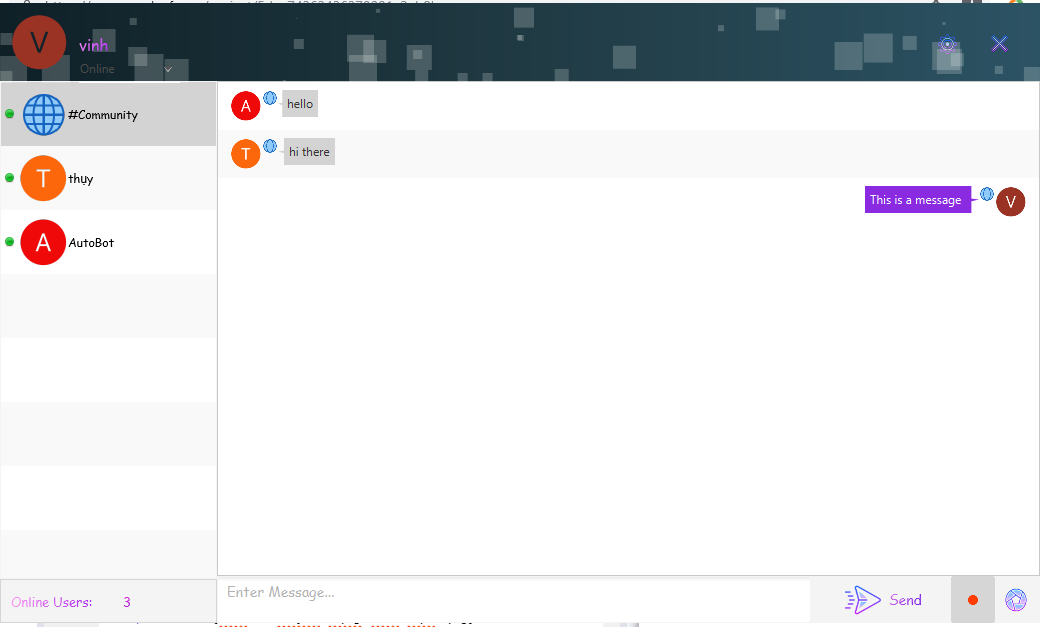
\includegraphics[scale=0.5]{send-voice-message.PNG}
			\caption{Send voice message}
			\label{fig:my_label}
		\end{figure}
		\item Nhấn vào nút thu âm 1 lần nữa để gửi đi. Kết quả như hình sau.
		\begin{figure}[H]
			\centering
			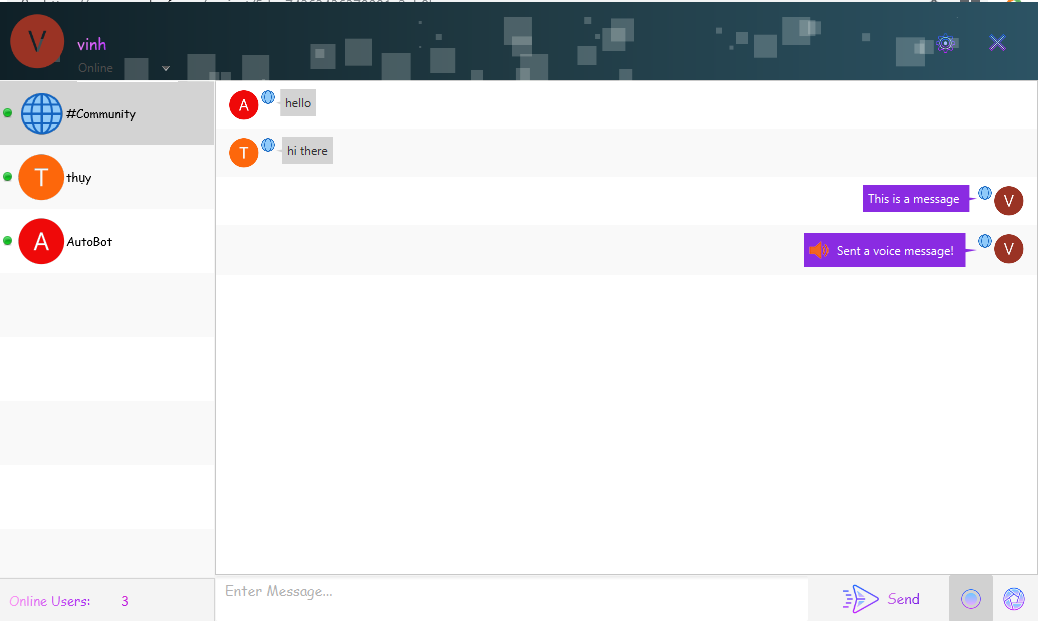
\includegraphics[scale=0.5]{voice-message.PNG}
			\caption{Voice message sent}
			\label{fig:my_label}
		\end{figure}
		\item Để gửi file nhấn vào nút duyệt file bên phải nút thu âm để mở hộp thoại chọn thư mục.
		\begin{figure}[H]
			\centering
			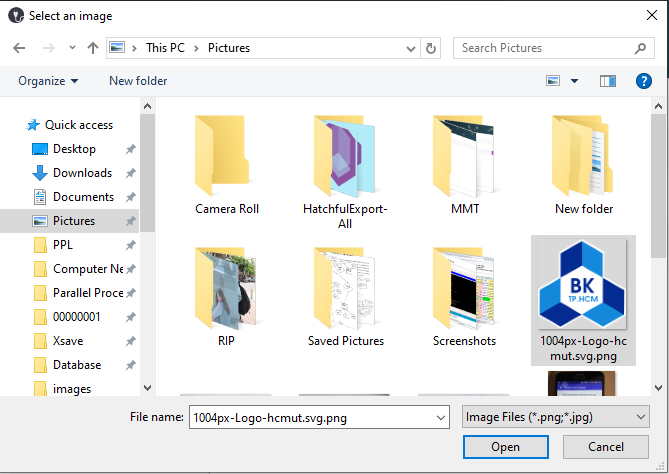
\includegraphics[scale=0.5]{send-file.PNG}
			\caption{Browse file}
			\label{fig:my_label}
		\end{figure}
		\item Nhấn vào file cần chọn. Kết quả như hình sau.
		\begin{figure}[H]
			\centering
			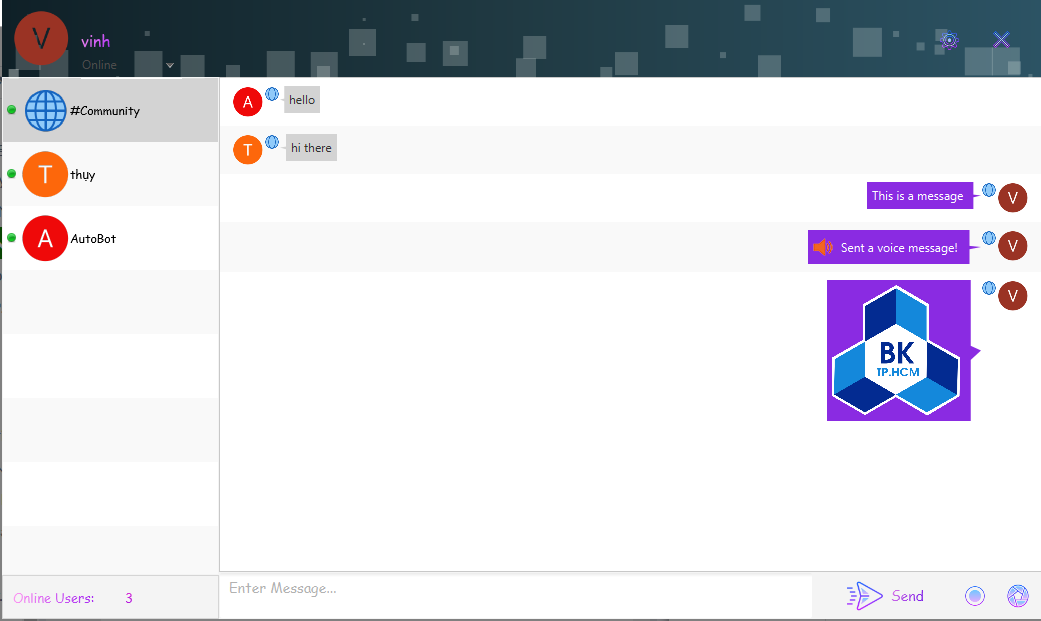
\includegraphics[scale=0.5]{file-sent.PNG}
			\caption{File sent}
			\label{fig:my_label}
		\end{figure}
	\end{itemize}
	\subsubsection{Gửi tin nhắn riêng cho user khác}
	\begin{itemize}
		\item Nhấp chọn user để gửi tin nhắn đến.
		\item Cửa sổ chat mới hiện ra.     
		\begin{figure}[H]
			\centering
			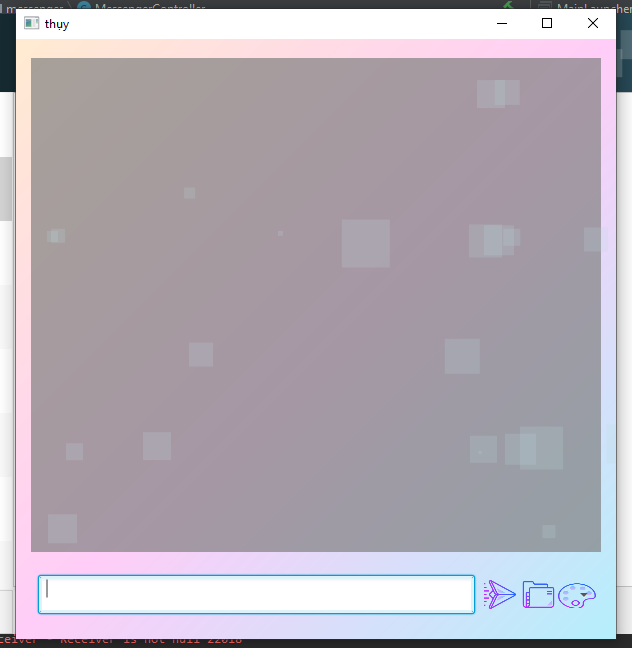
\includegraphics[scale=0.5]{start-chat-private.PNG}
			\caption{Send private message}
			\label{fig:my_label}
		\end{figure}
		\item Nhập tin nhắn từ bàn phím vào ô chat dưới cùng.
		\begin{figure}[H]
			\centering
			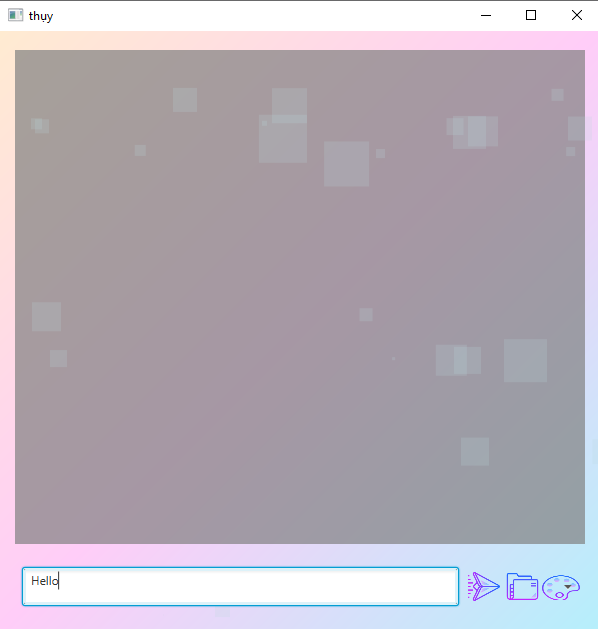
\includegraphics[scale=0.5]{enter-message-private.PNG}
			\caption{Enter private message}
			\label{fig:my_label}
		\end{figure}
		\item Nhấn nút send hình máy bay giấy ở bên cạnh ô chat hoặc nhấn phím enter để gửi tin.
		\begin{figure}[H]
			\centering
			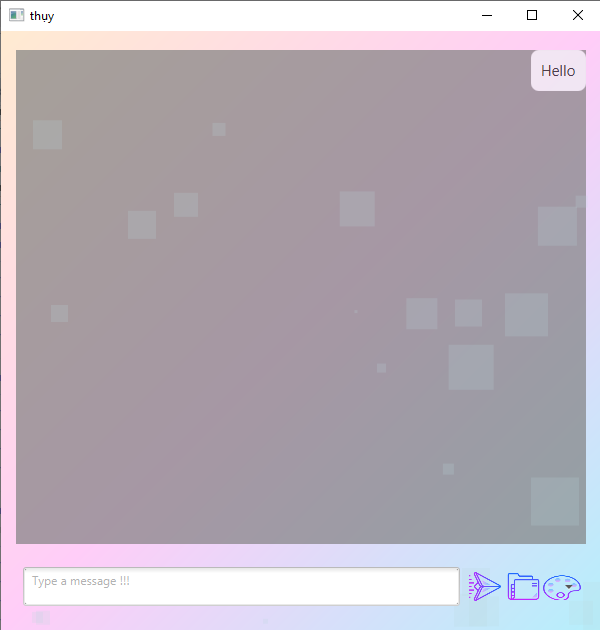
\includegraphics[scale=0.5]{message-sent-private.PNG}
			\caption{Private message sent}
			\label{fig:my_label}
		\end{figure}
		\item Để gửi tệp tin nhấn nút hình tệp tin cạnh nút send để mở hộp thoại chọn thư mục.
		\begin{figure}[H]
			\centering
			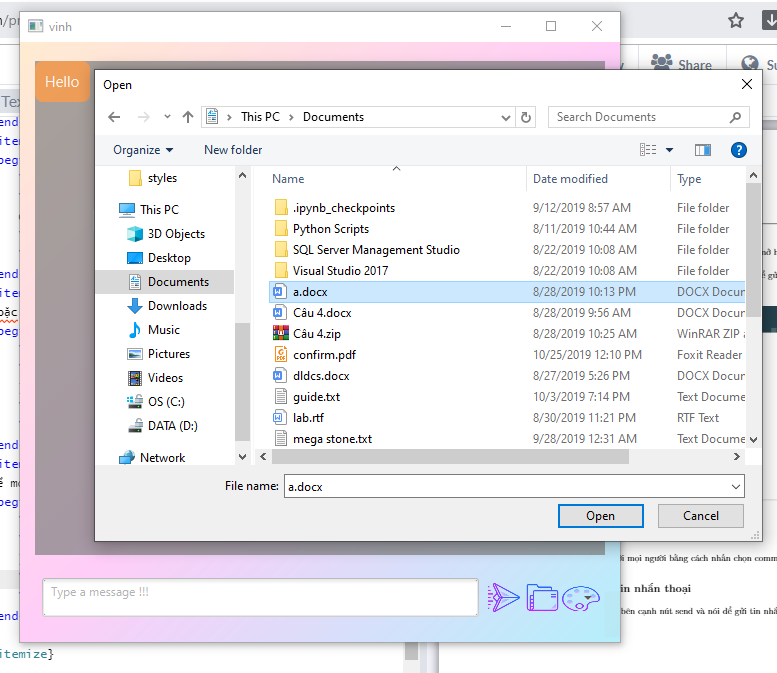
\includegraphics[scale=0.5]{browse-directory-private.PNG}
			\caption{Browse directory private}
			\label{fig:my_label}
		\end{figure}
		\item Nhấn open để gửi. Kết quả như hình sau.
		\begin{figure}[H]
			\centering
			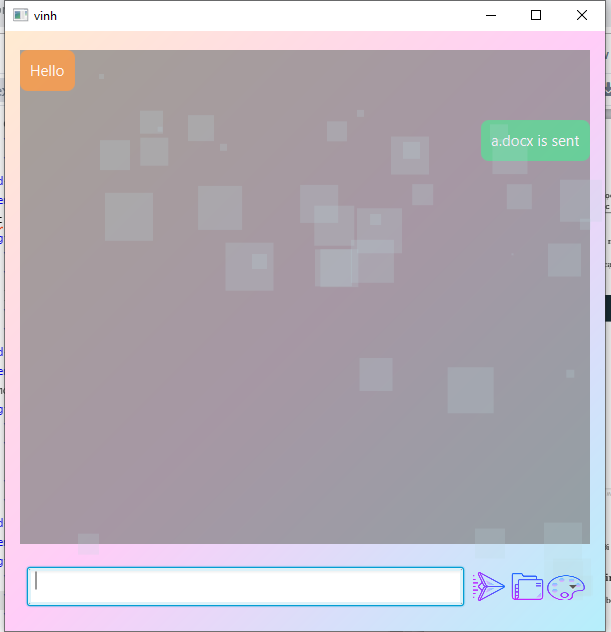
\includegraphics[scale=0.5]{private-file-sent.PNG}
			\caption{Private file sent}
			\label{fig:my_label}
		\end{figure}
		\item Để đồi màu bóng chat nhấn chọn nút bảng màu nằm bên phải nút chọn file và chọn màu.
		\begin{figure}[H]
			\centering
			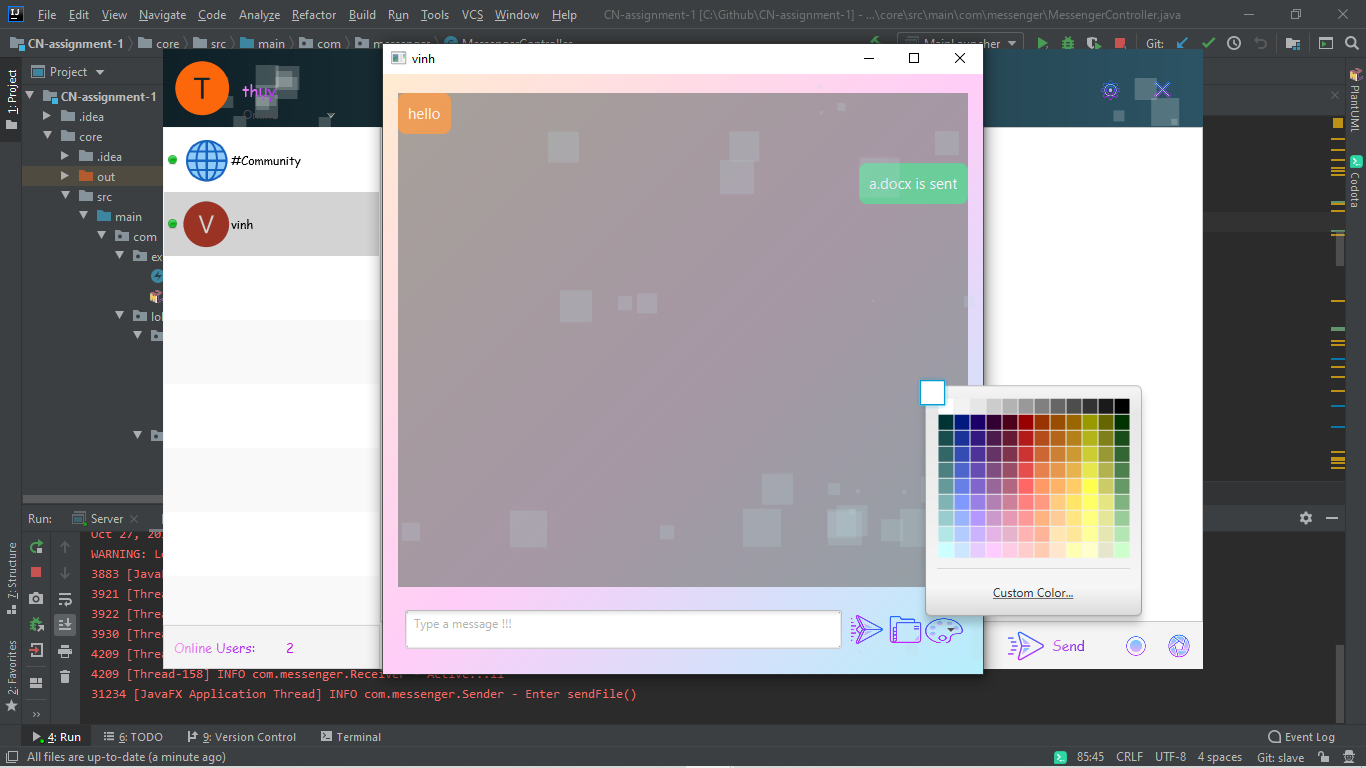
\includegraphics[width=\linewidth]{browse-color.png}
			\caption{Change chat bubble's color}
			\label{fig:my_label}
		\end{figure}
		\item Kết quả như hình sau.
		\begin{figure}[H]
			\centering
			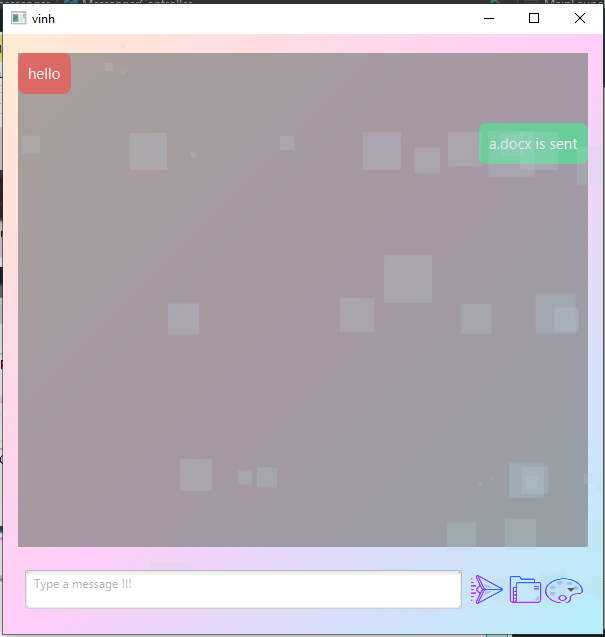
\includegraphics[scale=0.5]{color-changed.PNG}
			\caption{Chat bubble's color changed}
			\label{fig:my_label}
		\end{figure}
	\end{itemize}
	\subsection{Bước 4: Chuyển trạng thái hoạt động}
	Nhấn vào dấu mũi tên ở dưới username góc trên cùng bên trái để mở bảng chuyển trạng thái.
	\begin{figure}[H]
		\centering
		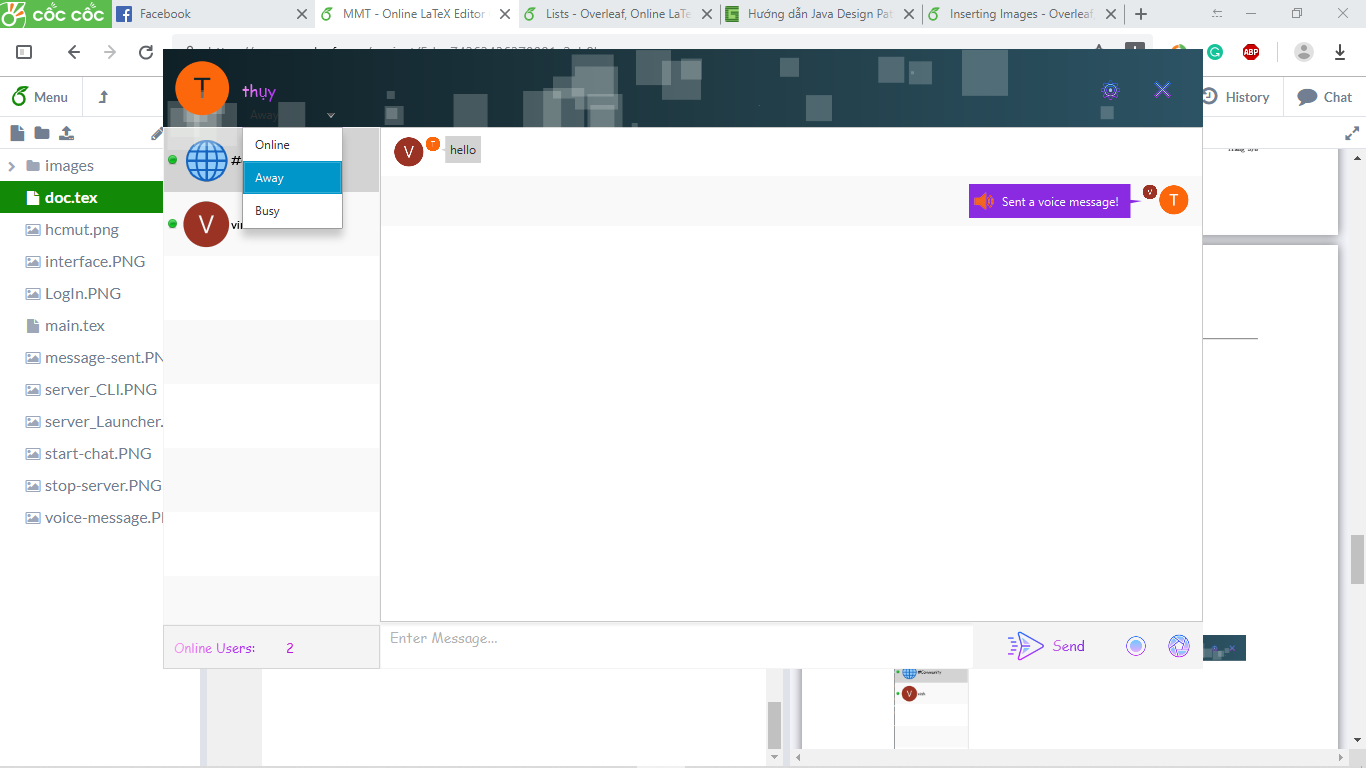
\includegraphics[width=\linewidth]{state-change.png}
		\caption{Change state}
		\label{fig:my_label}
	\end{figure}
	Sau khi đổi trạng thái, dấu tích ở bên cạnh username sẽ đổi màu đối với các user khác.
	\begin{figure}[H]
		\centering
		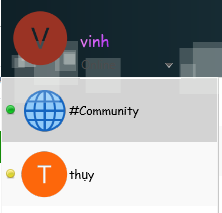
\includegraphics[scale=0.5]{state-changed.PNG}
		\caption{State changed}
		\label{fig:my_label}
	\end{figure}


\end{document}